
\subsection{Декодеривание}

\begin{frame}[t] % [plain]
	\begin{columns}
		\begin{column}{6.5cm}
			\graybox{Декодер}{
				\begin{center}
					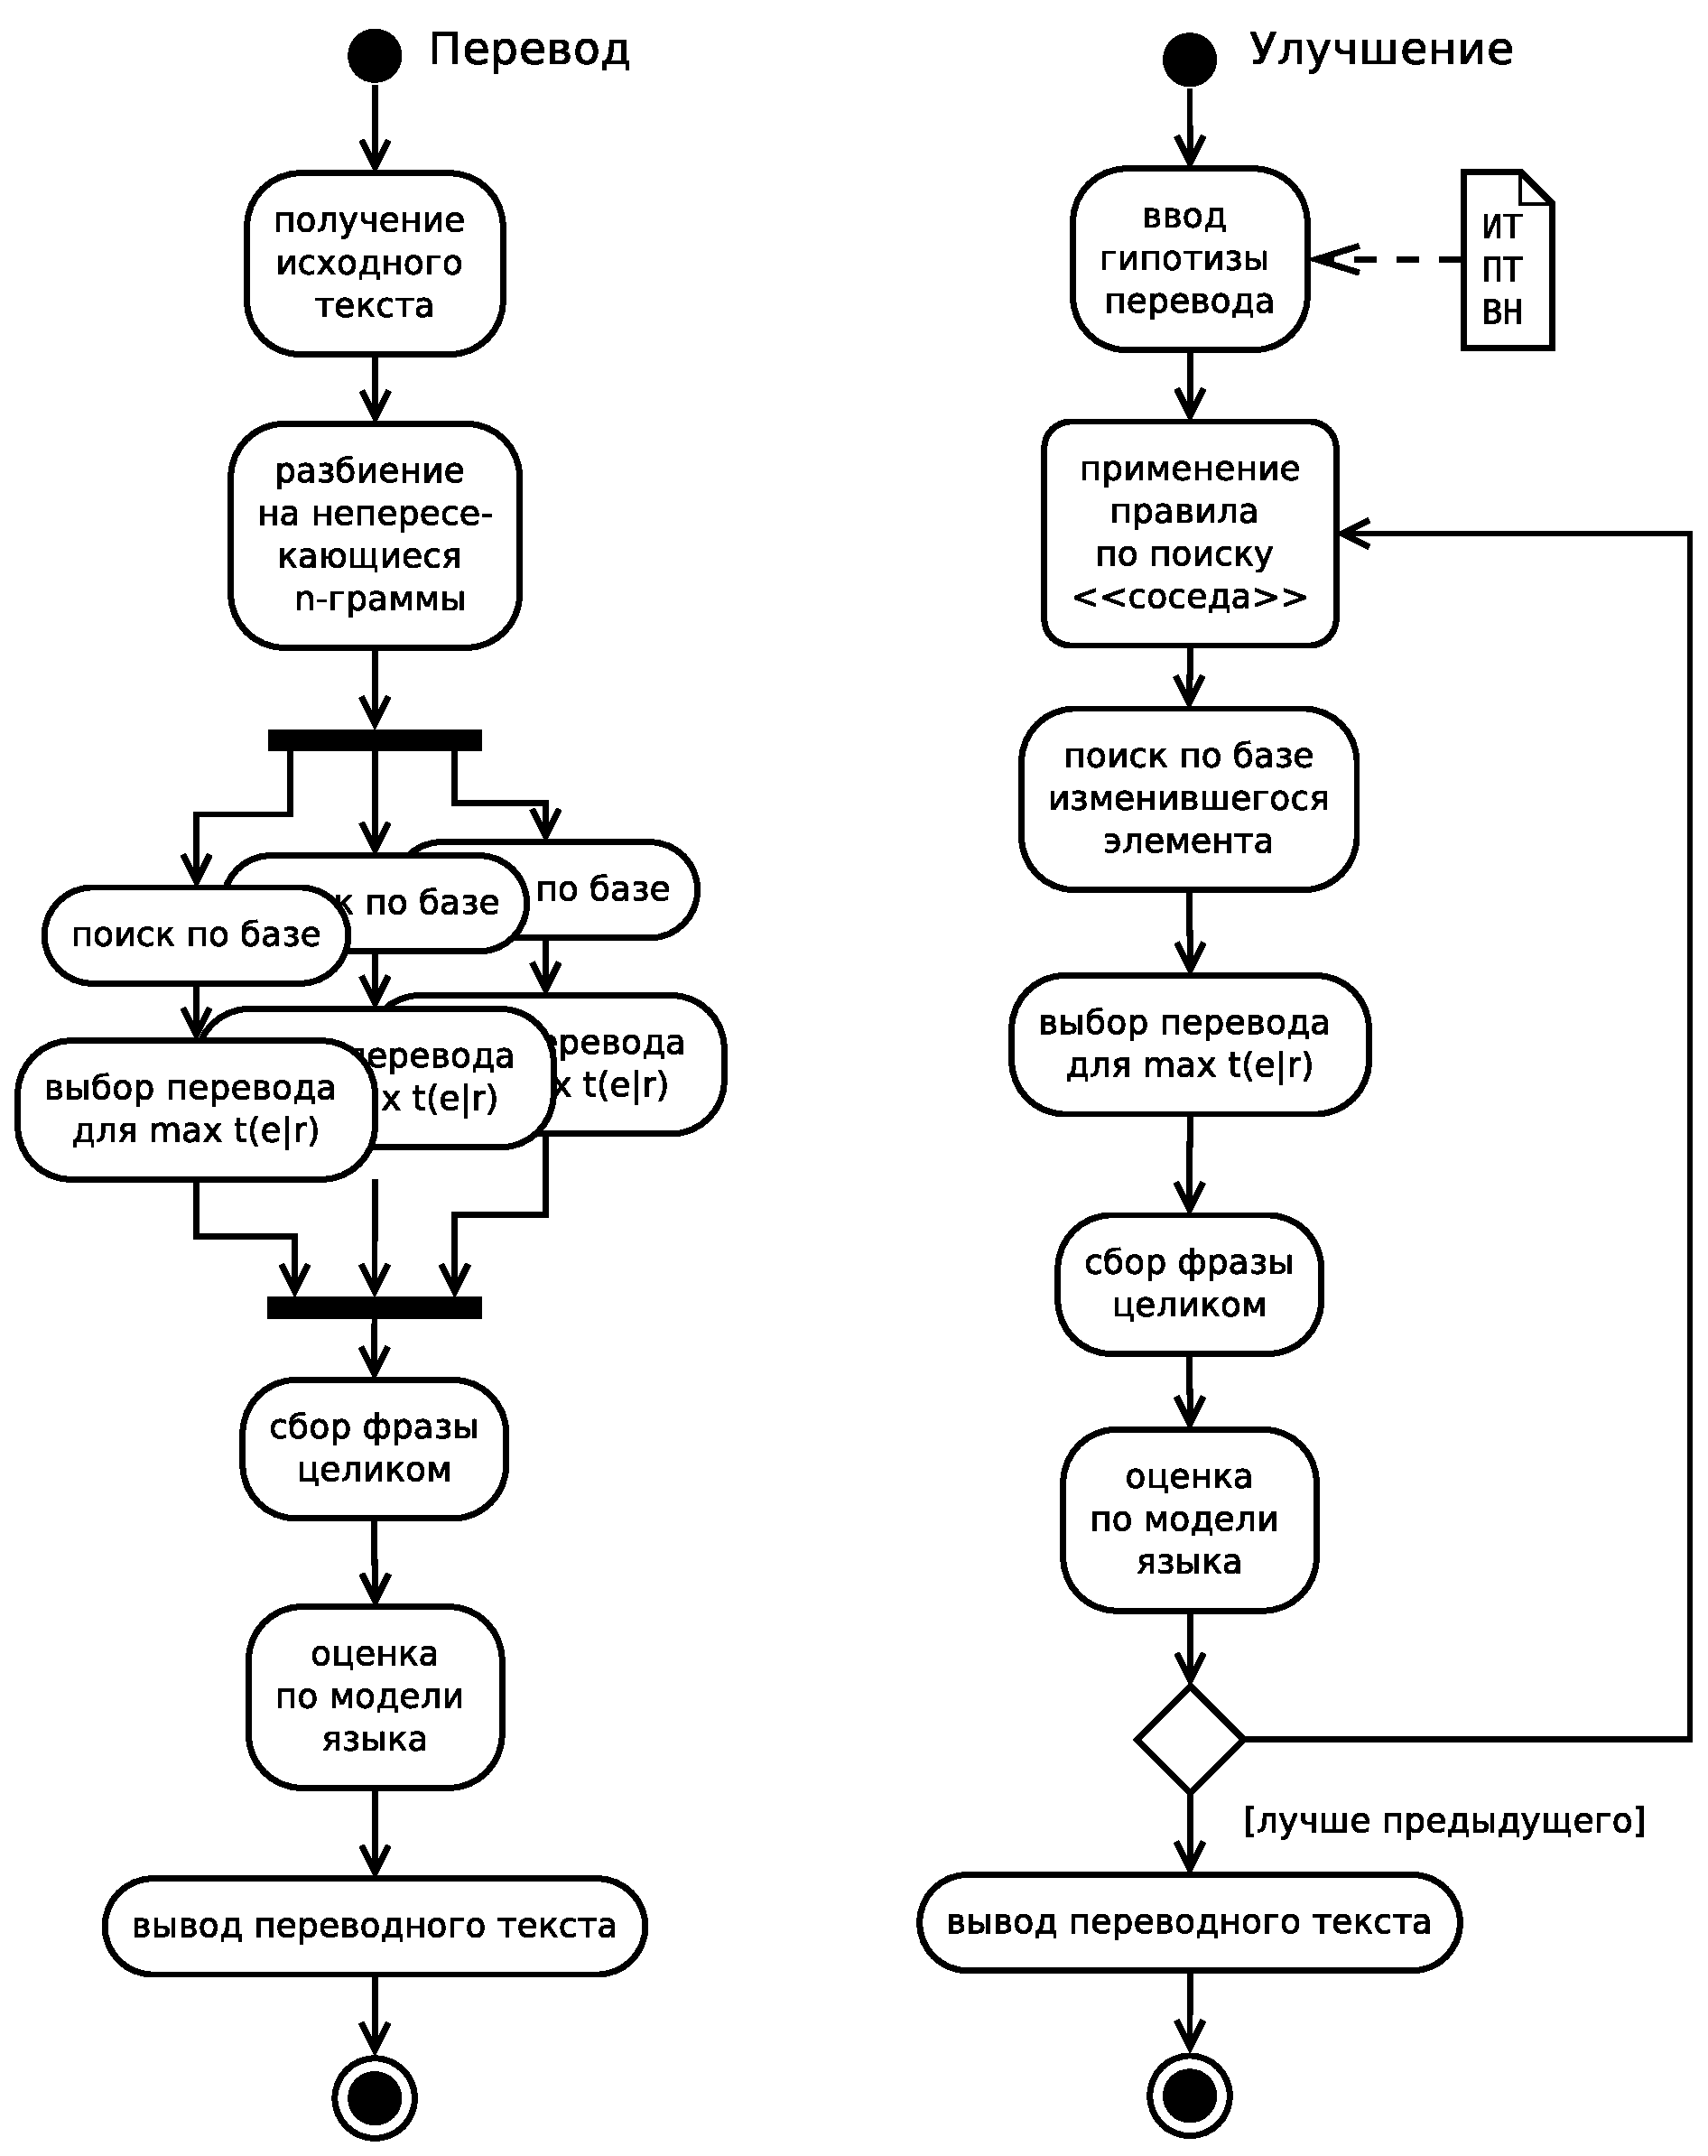
\includegraphics[height=7.5cm]{./vec/arch-decoder.eps}
				\end{center}
			}
		\end{column}
		\begin{column}{5cm}
			\small
			\begin{itemize}
				\item жадный инкрементный поиск;
				\item два режима работы:
				\begin{itemize}
					\item перевода,
					\item улучшения.
				\end{itemize}
				\item пошаговый веб-интерфейс;
				\item потоковый RESTful-сервис;
				\item пошаговый консольный интерфейс.
			\end{itemize}
		\end{column}
	\end{columns}
\end{frame}
